% !TeX spellcheck = en_US
\section{Evaluation of the VAS}
\label{sec:730_evaluation}
The evaluation of \ac{VAS} is structured into two parts. 
First, the possible data traffic reductions and then the quality gains when applying \ac{VAS}'s adaptation schemes are evaluated in a prototypical evaluation setup. Then, subjective user studies are used to assess the impact of the proposed adaptation schemes on the streaming experience.
\subsection{Objective Analysis of VAS's Adaptation Schemes}
\label{sec:730_evaluation_objective_analysis}
The data required for streaming video is determined in this section for \ac{VAS}'s adaptation schemes in comparison to state-of-the-art algorithms and the optimal adaptation scheme proposed in Section~\ref{sec:726_optimalAdaptation}. 
\subsubsection{Setup of the Evaluation}
\label{sec:730_evaluation_objective_analysis_setup}
This section describes the experimental setup using a prototypical implementation of the concepts discussed in previous sections.
The first paragraph of this section shows the physical setup, with mobile devices receiving video streams as well as network traces used for mimicking different real streaming sessions.

To mimic a real deployment of \ac{VAS} as a support service, different state-of-the-art adaptation schemes are implemented for the \ac{MPEG} \ac{DASH} reference client, DASH.js\footnote{https://github.com/Dash-Industry-Forum/dash.js; Visited on: 06/30/2016}.
The used adaptation schemes are discussed in the second paragraph.

The third paragraph describes the used  \ac{MPEG} \ac{DASH} videos with different content characteristics specific for this evaluation.
\paragraph{Setup of the Network Experiments}
The evaluation setup consists of the prototypical implementation of \ac{VAS}, a video hosting server, and three mobile devices (Google Nexus 5) that receive the video streams.
Wireless connections are available between all devices using an IEEE 802.11g access point.
Mobile Android devices allow us to use the full network stack of a mobile device. 
The setup is depicted in Figure~\ref{fig:network_setup}.
\begin{figure}[!tbh]
\centering
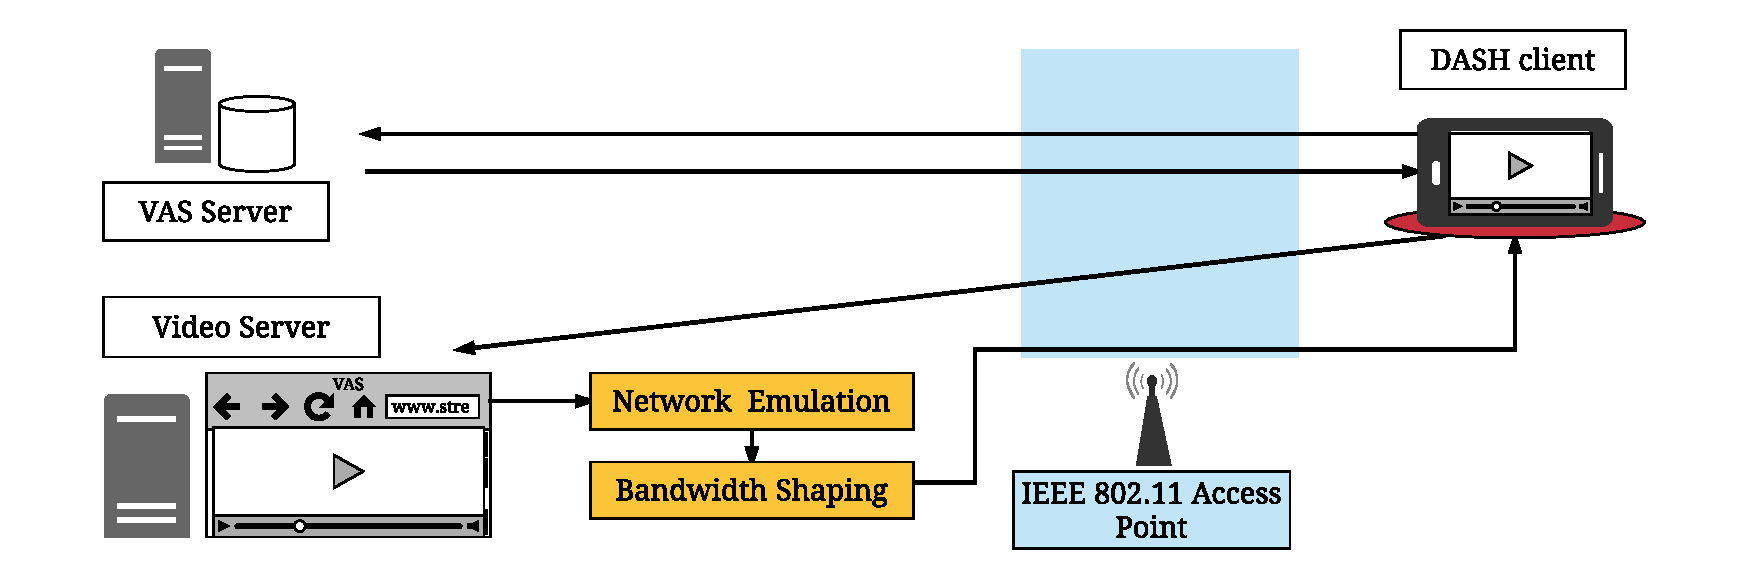
\includegraphics[width=\linewidth]{./gfx/700_VAS/setup}
\caption[Evaluation setup for \ac{VAS}]{Evaluation setup for the \ac{VAS} which shapes the data traffic for video segment delivery.}
\label{fig:network_setup}
\end{figure}

A single Ubuntu 14.04 server is used to host a web server that provides \ac{VAS} and various videos.
Even though the web server and \ac{VAS} run on the same physical machine, they do not exchange any information locally.
The quality models are generated online using the \ac{RT-VQM} algorithm, which is run on three different Amazon Web Service (AWS) machines of type "g2.2xlarge"\footnote{Intel Xeon E5-2670 \ac{CPU} with 16GB of memory and dedicated NVIDIA GRID \ac{GPU}s with 1536 \ac{CUDA} cores.}~\cite{Wichtlhuber2016}.
Using the IEEE 802.11g access point, any VAS-enabled client can communicate without limitations with VAS.

Requests to the web server are not restricted, but \ac{MPEG} \ac{DASH} segments underlie a traffic shaping component for both the respective throughput and the latency.
To mimic real streaming sessions and allow reproducible results, openly available network traces gathered by Eittenberger et al. and Riiser et al. are input for a traffic-shaping component on the server~\cite{Eittenberger2013,Riiser2013}.
The throughput and latency on the path from the video server is limited on a per-client basis. 
Eittenberger et al.'s traces are based on monitoring YouTube streaming sessions in the \ac{UMTS} network in the area of Bamberg, Germany.
The network traces are sampled in an interval of 10 seconds in the network of the mobile operator T-Mobile using two different mobile Android devices (Huawei S7-301u MediaPad, Samsung Galaxy Tab GT-P1000).
\begin{figure}[!htb]
\centering
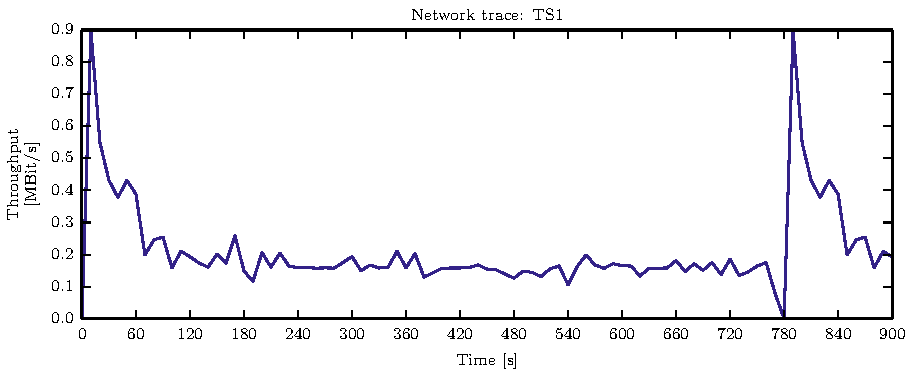
\includegraphics{./gfx/700_VAS/plotTraces_TS1}
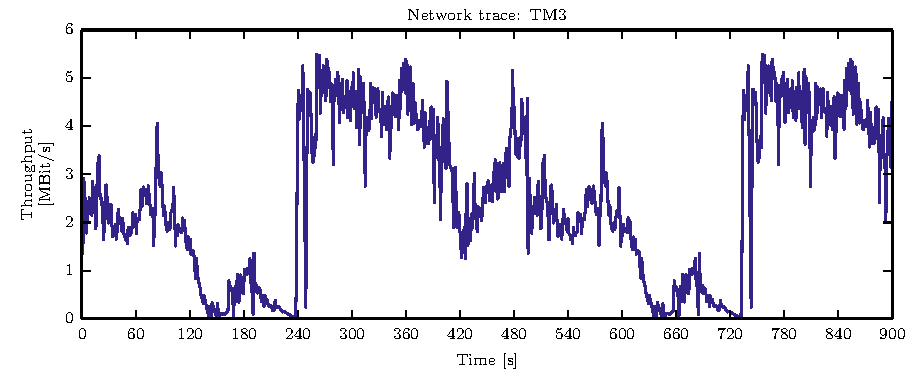
\includegraphics{./gfx/700_VAS/plotTraces_TM3}
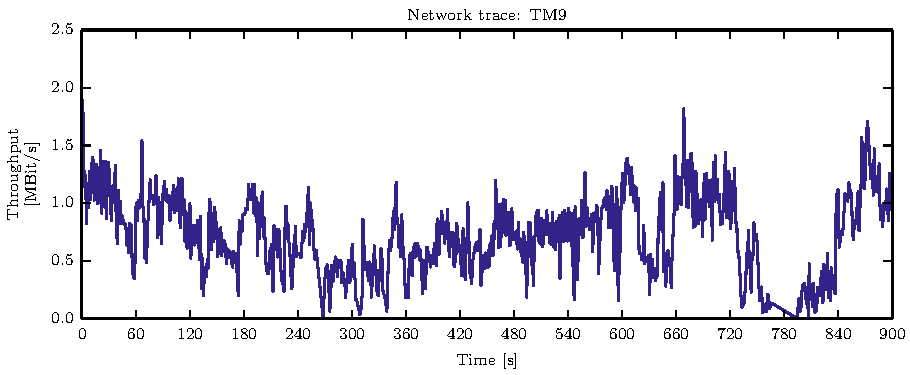
\includegraphics{./gfx/700_VAS/plotTraces_TM9}
\caption[Example network traces used for the VAS evaluation]{Network traces TS1 from Eittenberger et al.'s dataset~\protect\cite{Eittenberger2013} and 
TM3, TM9 of Riiser et al.~\cite{Riiser2013} are shown for the first 900 seconds of a streaming session.}
\label{fig:730_plotTOMMTraces}
\end{figure}
Two traces include video streaming sessions of a moving device with a speed of up to 50 km/h (TM1 and TM2) on a track of 3.6 km in the city center.
The average throughput of the trace is 0.258 \unit{$\frac{MBit}{s}$} for TM1 and 0.822 \unit{$\frac{MBit}{s}$} for TM2.
Two other traces are created with static device positions that show average throughputs of 0.194 \unit{$\frac{MBit}{s}$} for TS1 and 0.569 \unit{$\frac{MBit}{s}$} for TS2.
One additional, synthetic trace with a constant throughput of 90 \unit{$\frac{MBit}{s}$} (TO1) was added, which depicts mobile streaming under ideal conditions.

The network traces of Riiser et al.~\cite{Riiser2013} include mobile streaming sessions in 3G networks in Northern Europe. 
The sessions are captured using the proprietary Opera Netview Media Client on Laptops using a Huawei Model E1752 HSPA USB stick, while streaming video from a dedicated video server.
The trace is sampled approximately every second.
The video streaming sessions used a \ac{HAS} protocol for streaming video.
Different vehicles are used including, bus, metro, tram, and car. 
The traces' average throughputs are depicted in Table~\ref{tab:730_traces}.

For each evaluation run, a starting point of the trace is randomly selected while keeping the trace's characteristics. 
Ten evaluation runs are conducted for each video sequence and trace while its main characteristics - the average throughput and variance - deviate only slightly. 
At any time, a minimal throughput of 1 \unit{$\frac{KBit}{s}$} is guaranteed.
The traces are tailored so that the throughput shaping is refreshed every $200$ milliseconds.
If the streaming session lasts longer than the available trace duration, the trace is repeated. 
\begin{table}[!htb]
	\centering
	\caption{Overview of the network traces used for evaluating \ac{VAS}.}
	\begin{tabular}{c|cccc}
	\toprule[2.0pt]
	\textbf{ID} &  \textbf{Application} & \textbf{Category} & \textbf{Duration} & \textbf{Avg. throughput}  \\ 
	\hline
	\multicolumn{5}{l}{\textbf{Eittenberger et al.~\cite{Eittenberger2013}}}\\
	\hline
	TM1 & YouTube & Mobile (Car) & 12:13 min & 0.258 Mbit/s \\
	TM2 & YouTube & Mobile (Car) & 6:39 min & 0.822 Mbit/s \\
	TS1 & YouTube & No Mobility & 12:42 min &  0.194 Mbit/s \\
	TS2 & YouTube & No Mobility & 10:26 min & 0.569 Mbit/s \\
	\hline
	\multicolumn{5}{l}{\textbf{Riiser et al.~\cite{Riiser2013}}}\\
	\hline
	TM3 & Opera Netview & Mobile (Bus) & 8:14 min & 2.765 Mbit/s \\
	TM4 & Opera Netview & Mobile (Bus) & 22:44 min & 2.617 Mbit/s \\
	TM5 & Opera Netview & Mobile (Bus) & 9:47 min & 1.992 Mbit/s \\
	TM6 & Opera Netview & Mobile (Bus) & 7:24 min & 2.447 Mbit/s \\
	TM7 & Opera Netview & Mobile (Metro) & 3:15 min & 1.451 Mbit/s \\
	TM8 & Opera Netview & Mobile (Metro) & 17:10 min & 0.584 Mbit/s \\
	TM9 & Opera Netview & Mobile (Tram) & 23:48 min & 0.777 Mbit/s \\
	TM10 & Opera Netview & Mobile (Tram)& 23:27 min & 0.921 Mbit/s \\
	TM11 & Opera Netview & Mobile (Tram) & 25:11 min & 0.679 Mbit/s \\
	TM12 & Opera Netview & Mobile (Tram) & 21:13 min & 0.791 Mbit/s \\
	TM13 & Opera Netview & Mobile (Tram) & 25:09 min & 0.838 Mbit/s \\
	TM14 & Opera Netview & Mobile (Ferry) & 19:22 min & 1.568 Mbit/s \\
	TM15 & Opera Netview & Mobile (Ferry) & 9:15 min & 1.829 Mbit/s \\
	TM16 & Opera Netview & Mobile (Car) & 123:20 min & 0.727 Mbit/s \\
	TM17 & Opera Netview & Mobile (Car) & 203:44 min & 0.726 Mbit/s \\
	TM18 & Opera Netview & Mobile (Car) & 7:16 min & 1.761 Mbit/s \\
	TM19 & Opera Netview & Mobile (Train) & 40:42 min & 1.393 Mbit/s \\
	TM20 & Opera Netview & Mobile (Train) & 36:42 min & 1.123 Mbit/s \\
	\hline
	\multicolumn{5}{l}{\textbf{Artificial}}\\
	\hline
	TO1 & - & No Mobility & 60:00 min & 90 Mbit/s \\
	\bottomrule[2.0pt]
	\end{tabular} 
	\label{tab:730_traces}
\end{table}
\paragraph{Adaptation Schemes}
\label{sec:730_BufferApproaches}
\ac{VAS} is designed to support any existing \ac{MPEG} \ac{DASH} adaptation scheme, which fulfills the requirements discussed in Section~\ref{sec:726_adaptation_strategies}.
For making adaptation decisions, those schemes rely either on  playback buffer information or a measurement of  the current application-layer throughput.
Schemes using the playback buffer analyze the playback buffer fill state, i.e., the ratio between the available video segments in the playback buffer in seconds and the size of the playback buffer in seconds.

Different state-of-the-art schemes of both categories are implemented. These are selected either from an experimental study of Thang et al. or from widely used \ac{MPEG} \ac{DASH} streaming clients~\cite{Thang2014}.
The \emph{\ac{TBB}} scheme assumes that a playback buffer is split into zones, which are defined by thresholds that initiate different adaptation behaviors.
The $T_{B_{c}}$ represents the critical zone of the buffer, $T_{B_{l}}$ defines the zone in which the buffer fill state is perceived as low; $T_{B_{n}}$ is the desired buffer fill state and $T_{B_{max}}$ shows the buffer capacity.
In this evaluation, the approach of Miller et al. is used in which a  buffer fill state between $T_{B_{c}}$ and $T_{B_{l}}$ adapts to the next lower representation index~\cite{Miller2012}.
A buffer fill state below $T_{B_{c}}$ initiates an adaptation to the lowest representation.
The adaptation scheme maintains the current representation as long as the buffer fill state is between $T_{B_{l}}$ and $T_{B_{n}}$, while the representation index is increased when the buffer fill state is above $T_{B_{n}}$.

A \emph{\ac{TB}} measures the current throughput of the network on the application layer and decides when and how to adapt based on this measurement~\cite{Thang2012}.
The \ac{MPEG} \ac{DASH} representation to download is determined by its bit rate, which should be equal or below the current throughput of the network. 
The \ac{TB} may lead to disturbing oscillation effects if the measured throughput suffers from adaptation oscillations. 
An approach to mitigate peaks in the measured throughput is to use the \emph{\ac{ST}} as: $TP_{smooth}(t) = ((1 - \rho) * TP(t-1) +  \rho * TP(t)) * (1-\beta)$, where $\rho$ represents the weight between $t-1$ and $t$ and $\beta$ is a safety margin.
$t$ and $t-1$ are measured as the average throughput after the download of a complete \ac{MPEG} \ac{DASH} segment.

Combinations of throughput-based and buffer-based adaptation schemes are proposed, e.g., with Miller's \emph{\ac{BTR}}~\cite{Miller2012}. 
\ac{BTR} triggers adaptations according to the thresholds of the \ac{TBB}, but determines the representation to switch to depending on the current throughput.

Akhshabi et al. show another hybrid method relying on the \ac{ST} and the buffer levels $T_{B_{c}}$ and $T_{B_{l}}$, which is called \emph{\ac{TBST}}~\cite{Akhshabi2011}. 
For a buffer fill state below $T_{B_{c}}$ the lowest representation is chosen.
In contrast, an adaptation to the next lower bit rate is performed if the measured throughput is below the current representation bit rate and the buffer fill state is between $T_{B_{c}}$ and $T_{B_{l}}$.
Similarly, when above $T_{B_{l}}$ the representation index is increased by one, if the smoothed throughput is stable or increasing and the next representation's bit rate is below the smoothed throughput. 
This adaptation scheme smoothly adapts when the available throughput changes. 
The method is called threshold-based smoothed throughput measurement adaptation (TBSTA).

M\"uller et al. propose a hybrid model (\ac{ATB})~\cite{Muller2012}.
\ac{ATB} performs an aggressive adaptation where a buffer fill state below $T_{B_{c}}$ triggers an adaptation to a representation with a bit rate which is below 0.3 times the current throughput. A buffer fill state between $T_{B_{c}}$ and $T_{B_{l}}$ defines the desired bit rate to be below half of the measured throughput, and a fill state between $T_{B_{l}}$, and  $T_{B_{n}}$ adapts to a bit rate equal or below the current throughput. 
Above $T_{B_{n}}$, the current throughput is multiplied by $\gamma$, where $\gamma > 1$, to determine the next representation.

The last scheme discussed is the \ac{QD}~\cite{Mok2012}, which aims for quality-aware streaming but neglects content characteristics during adaptation decisions. 
To improve the perceived quality, \ac{QD}~\cite{Mok2012} decreases the representation index if network conditions degrade. 
This behavior follows the same idea as the proposed \ac{SQA} scheme but is rather static, as the intermediate representation is chosen to be one index above the target representation.
If the network conditions allow a higher representation than the current one, a direct jump to the possible representation index is performed.  

All the above adaptation schemes are evaluated with and without support of the \ac{VAS} adaptation support. 
The optimal adaptation scheme is implemented using the optimization software Gurobi 6.5.2\footnote{http://www.gurobi.com/index; Visited on: 06/30/2016}.
\paragraph{Video Dataset}
\label{sec:730_video_dataset}
The videos used for evaluation are from the publicly available \ac{MPEG} \ac{DASH} datasets provided by Lederer et al. consisting of the sequences:
The Swiss Account (VTSA), Big Bucks Bunny (VBBB), Valkaama (VV), Of Forest and Men (VOFM), Redbull Playstreets (VRBPS), Tears of Steel (VTOS) and the Elephant's Dream (VED)~\cite{Lederer2013}.
The characteristics of frame rate, bit rate in \unit{$\frac{KBit}{s}$}, and resolutions for different \ac{MPEG} \ac{DASH} representations are shown in Table~\ref{tab:730_videos}.
\begin{table}[!htb]
\caption[Video encoding profiles used in the VAS evaluation]{Video encoding profiles of different videos from the \ac{MPEG} DASH dataset~\cite{Lederer2013} with static frame rates for each video and variable resolutions (S) and bit rates (B) in \unit{$\frac{KBit}{s}$}. R shows the \ac{MPEG} \ac{DASH} representation index.}
\resizebox{\textwidth}{!}{%
\begin{tabular}{c|cc|cc|cc|cc|cc|cc|cc}
\toprule[2.0pt]
& \multicolumn{2}{c}{\textbf{\specialcell{VBBB\\24$\unit{FPS}$}}} & \multicolumn{2}{c}{\textbf{\specialcell{VED\\24$\unit{FPS}$}}} & \multicolumn{2}{c}{\textbf{\specialcell{VOFM\\24$\unit{FPS}$}}} & \multicolumn{2}{c}{\textbf{\specialcell{VTOS\\24$\unit{FPS}$}}} & \multicolumn{2}{c}{\textbf{\specialcell{VTSA\\30$\unit{FPS}$}}} & \multicolumn{2}{c}{\textbf{\specialcell{VV\\30$\unit{FPS}$}}} & \multicolumn{2}{c}{\textbf{\specialcell{VRBPS\\30$\unit{FPS}$}}} \\
R &   \textbf{S} & \textbf{B}  & \textbf{S} & \textbf{B} &  \textbf{S} & \textbf{B} & \textbf{S} & \textbf{B}  & \textbf{S} & \textbf{B} & \textbf{S} & \textbf{B}  & \textbf{S} & \textbf{B}  \\ 
\hline
0 &  240p & 46 &  240p & 46 &  240p & 47 &  270p & 255 &  240p & 91 &  240p & 46 &  240p & 101 \\
1 &  240p & 89 &  240p & 91 &  240p & 91 &  360p & 508 &  240p & 131 &  240p & 88 &  240p & 151 \\
2 &  240p & 131 &  240p & 131 &  240p & 135 &  360p & 811 &  360p & 174 &  240p & 123 &  360p & 201 \\
3 &  360p & 178 &  360p & 180 &  360p & 186 &  544p & 1113 &  360p & 216 &  360p & 175 &  360p & 251 \\
4 &  360p & 222 &  360p & 222 &  360p & 232 &  720p & 1516 &  360p & 257 &  360p & 214 &  360p & 301 \\
5 &  360p & 263 &  360p & 261 &  360p & 277 &  720p & 2427 &  360p & 337 &  360p & 250 &  480p & 501 \\
6 &  360p & 334 &  360p & 328 &  360p & 366 &  1080p & 3020 &  480p & 431 &  360p & 310 &  480p & 600 \\
7 &  360p & 396 &  360p & 382 &  480p & 462 &  1080p & 4028 &  480p & 602 &  480p & 439 &  480p & 700 \\
8 &  480p & 522 &  480p & 523 &  480p & 553 &  1080p & 6045 &  480p & 764 &  480p & 516 &  480p & 896 \\
9 &  480p & 595 &  480p & 594 &  480p & 644 &  1080p & 10068 &  480p & 967 &  480p & 587 &  480p & 1180 \\
10 &  720p & 791 &  720p & 796 &  576p & 825 &  &  &  720p & 1318 &  720p & 812 &  720p & 1499 \\
11 &  720p & 1033 &  720p & 1033 &  576p & 1006 &  &  &  720p & 1727 &  720p & 989 &  720p & 1994 \\
12 &  720p & 1245 &  720p & 1231 &  576p & 1268 &  &  &  720p & 2056 &  720p & 1237 &  720p & 2475 \\
13 &  720p & 1547 &  720p & 1495 &  576p & 1519 &  &  &  1080p & 2714 &  &  &  1080p & 2996 \\
14 &  1080p & 2134 &  1080p & 2118 &  576p & 1765 &  &  &  1080p & 3500 &  &  &  1080p & 3993 \\
15 &  1080p & 2484 &  1080p & 2445 &  576p & 2159 &  &  &  1080p & 3995 &  &  &  1080p & 4982 \\
16 &  1080p & 3079 &  1080p & 2980 &  576p & 2529 &  &  &  &  &  &  &  1080p & 5943 \\
17 &  1080p & 3527 &  1080p & 3431 &  576p & 3206 &  &  &  &  &  &  &  &  \\
18 &  1080p & 3840 &  1080p & 3791 &  &  &  &  &  &  &  &  &  &  \\

\bottomrule[2.0pt]
\end{tabular}}
\label{tab:730_videos}
\end{table}

These sequences are encoded using H.264/AVC, with a stable frame rate but varying resolutions and quantization parameters~\cite{Wiegand2003}.
The described dataset represents the common number of representations and encodings available for \ac{MPEG} \ac{DASH} streaming sessions, e.g., on YouTube or Netflix.
\acp{CDN} distribute even more representations than used in the \ac{MPEG} \ac{DASH} dataset. 
These representations differ in terms of their bit rates, resolutions, and frame rates and are available for different device categories~\cite{Krishnappa2015}.
Therefore, we transcode a video sequence into 60 representations with varying frame rates, resolutions and quantization levels. % and the recent H.265/HEVC encoding.
The result is the MPEG DASH video VHEVC, which is encoded in all combinations of spatial dimension (resolutions: 180p, 360p, 540p, 720p, 1080p), temporal dimension (frame rate: 15, 30, 45, 60 $\unit{FPS}$ ) and quality dimension (quantization: 21, 27, 33).
The bit rate of the lowest representation is 116.504 \unit{$\frac{KBit}{s}$}, the highest representation is 26.71 \unit{$\frac{MBit}{s}$}.

The video set used for evaluation offers a broad variety of structure, motion, and color information in order to show that \ac{VAS} achieves significant data traffic savings for different videos.
The videos differ in terms of the content features \ac{SI}, \ac{TI}, and \ac{Co}.
Figure~\ref{fig:730_picssiti} shows histograms on a subset of five videos (VBBB, VED, VOFM, VTOS, and VTSA).
The features are calculated per video shot and the occurrence of the feature values are normalized between 0 and 1.
Figure~\ref{fig:730_picssiti} illustrates that the video shots cover a broad range of the feature spectrum.
\begin{figure}
	\centering
	\subfloat{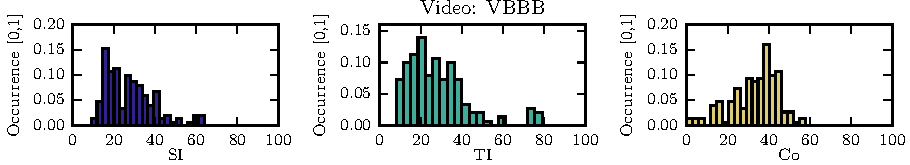
\includegraphics{./gfx/700_VAS/siti_histogram_videoVBBB}}\\
	\subfloat{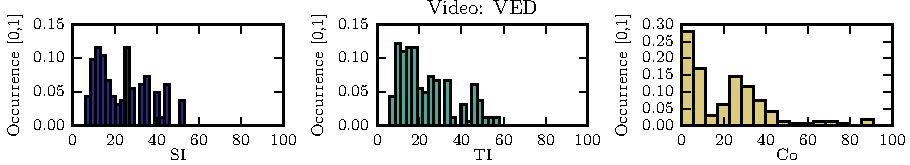
\includegraphics{./gfx/700_VAS/siti_histogram_videoVED}}\\
	\subfloat{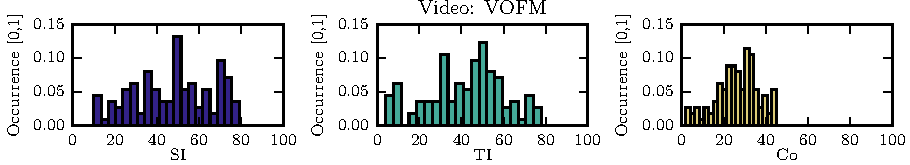
\includegraphics{./gfx/700_VAS/siti_histogram_videoVOFM}}\\
	\subfloat{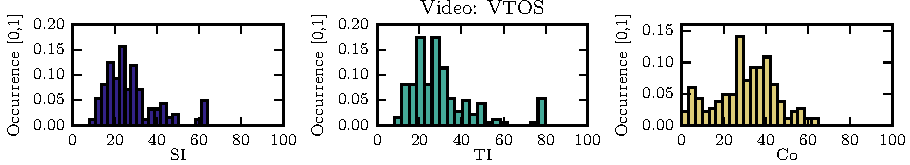
\includegraphics{./gfx/700_VAS/siti_histogram_videoVTOS}}\\
	\subfloat{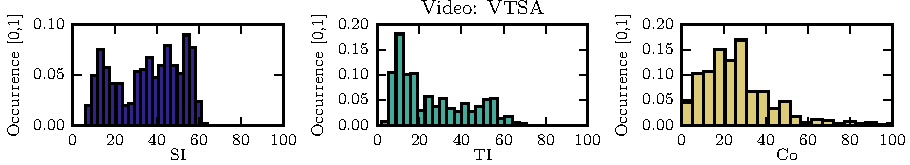
\includegraphics{./gfx/700_VAS/siti_histogram_videoVTSA}}\\
	\caption[Classification of the videos used for evaluation]{Classification of test videos regarding SI, TI, and Co.}
\label{fig:730_picssiti}
\end{figure}
\subsubsection{Data Traffic Reduction}
\label{sec:730_eval_network}
This section describes the achieved data traffic reductions using \ac{VAS} for different adaptation schemes.
The metric used for assessing data traffic reductions is the relative data traffic generated ($Q = \frac{DT_{VAS,AS}}{DT_{AS}}$), where $DT$ represents the amounts of bits transferred. $VAS,AS$ indicates that a \ac{VAS} scheme is used, whereas $AS$ indicates a non-\ac{VAS} scheme.
The relative data traffic reductions are expressed as $R = 1 - Q$.
\paragraph{Different Adaptation Schemes}
Using \ac{VAS} allows streaming clients to specify a target quality for adapting video.
In contrast to bit rate-based adaptation, this does not mean that the highest bit rate representation is always streamed.
This offers the potential to save data traffic.

A first scenario describes how much data traffic can be saved for a common mobile streaming client in an overcapacity scenario (network trace: TO1) for all videos.
For TO1, all evaluated schemes will eventually adapt to the highest bit rate representation, while \ac{VAS} solely adapts towards the lowest bit rate representation offering the desired quality.
For this scenario, the target quality is set to an \ac{MOS} of 5, representing the highest available quality of a video stream.
The remaining parameters are kept static for this evaluation: \ac{HTTP} Partial Get: Off, Playback Buffer Length: 20 seconds, Segment Duration: 2 seconds, and Session Time: 60 minutes\footnote{The segment length has been studied with values of \textbf{$2$  $\unit{seconds}$}, $4$ $\unit{seconds}$, $6$ $\unit{seconds}$ and $10$ $\unit{seconds}$ and the playback buffer length of $4$ $\unit{seconds}$, $12$ $\unit{seconds}$ and \textbf{$20$ $\unit{seconds}$}. Small but significantly improved results could be achieved using a small segment length, i.e., $2$ $\unit{seconds}$, and a large playback buffer size ($20$ $\unit{seconds}$).}.

The results depicted in Figure~\ref{fig:730_trafficReductionOverprovisioning} show achieved data traffic quota ($Q$) for the three video sequences VTSA, VRBPS, and VHEVC - and all adaptation schemes.
Also, the optimal adaptation is depicted as a red, dotted line.

Obviously, in the overcapacity scenario the data traffic quotas for all adaptation schemes are similar, but the data saving potential is very diverse for different videos. 
As in an overcapacity scenario, none of the adaptation schemes invokes a quality decreasing adaptation.
Thus, \ac{TQA} and \ac{SQA} achieve a similar data traffic quota ($Q$).
For the evaluated \ac{MPEG} \ac{DASH} video sequences (see Table~\ref{tab:730_videos}), the data traffic quota is in the range of 17.17\% (HEVC) to 72.64\% (VRBPS), meaning that even for VRBPS at the highest target quality level, the data saving potential lies at around 27.36\%.
 For videos similar to HEVC that have a multitude of representations, different video dimensions allow adaptation across frame rate, resolution, and quantization level.
Those adaptation schemes achieve data savings of up to 82.83\%.
As external conditions are similar for all videos, data traffic ratio differences are related to the encoded content, especially the volatility of the content characteristics.
Especially, highly varying video sequences such as HEVC, VTOS, or VV achieve large data savings, whereas VOFM or VRBPS have a low number of video shots that are usually rather long. 
VRBPS achieves the smallest reduction of around 27.36\% due to the variability of motion, structure, and color characteristics being comparably low between different video shots (see Figure~\ref{fig:730_picssiti}). 
This effect is related to higher encoding efficiency if video characteristics stay similar over longer times. 
\ac{VAS} heuristics, such as \ac{TQA}, benefit from videos with more representations, and thus, more fine-granular adaptation options.
Another reason for high data traffic savings is the availability for high bit rate and resolution representations.
For example, the low maximum resolution and bit rate of VOFM (\ac{576p}, 4 \unit{$\frac{MBit}{s}$}) limits \ac{VAS}'s potential for data traffic reduction.
\begin{figure}[!htb]
 \centering
 \subfloat[][]{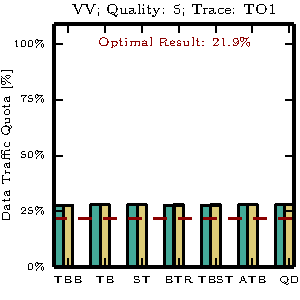
\includegraphics{./gfx/700_VAS/plotSavingsOptimal_TTTO1_TQ5_PG0_SL2001_BL20000_vid118}} % no legend
 \subfloat[][]{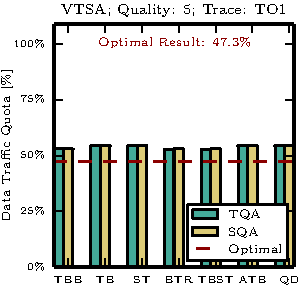
\includegraphics{./gfx/700_VAS/plotSavingsOptimal_TTTO1_TQ5_PG0_SL2001_BL20000_vid114}}
 \subfloat[][]{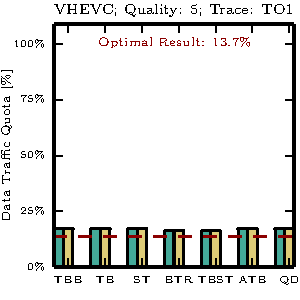
\includegraphics{./gfx/700_VAS/plotSavingsOptimal_TTTO1_TQ5_PG0_SL2001_BL20000_vid122}} %no legend
 \caption[Data traffic quota of using VAS's TQA and SQA]{Overview of the data traffic quota of VAS's TQA and SQA in relation to the pure adaptation scheme without VAS for the network trace TO1. The plots represent the videos % VBBB, VED, VOFM, VTSA, 
  (a) VV, (b) VTSA, and (c) VHEVC.}%, VTOS. }
 \label{fig:730_trafficReductionOverprovisioning}
\end{figure}

Also, the optimal adaptation is depicted for the videos VHEVC, VRBPS, and VTSA in Figure~\ref{fig:730_trafficReductionOverprovisioning}, and for all videos in Table~\ref{tab:730_trafficReductionOvercapacity}.
It is shown that the achieved data traffic quota of the adaptation scheme \ac{ATB} is close to the optimal adaptation.
Other adaptation schemes show similar results for the overcapacity trace (TO1).
On average, the difference between the proposed heuristics and the optimal adaptation in the overcapacity case ranges from 3.47\% to 7.14\%. 
\ac{VAS}'s heuristics are close to the optimal results achieved with global knowledge of the network trace and video characteristics.
Differences can be explained as the adaptation schemes supported by \ac{VAS} slowly adapt up to the highest quality representation in the beginning, whereas the global knowledge of the optimal adaptation allows an immediate switch to the highest quality. 
\ac{VAS}'s gap to the optimal adaptation is different for each video, as video representations differ in terms of bit rates, and \ac{VAS} is not aware of the video characteristics of future \ac{MPEG} \ac{DASH} segments. 
Again, \ac{VAS} heuristics such as \ac{TQA} benefit from videos with more representations and adaptation options in all three video dimensions. In the case of the HEVC sequence, the 60 encoded representations show a lower relative gap between the heuristics and the optimal adaptation.
\begin{table}[!h]
 \centering
 \caption[VAS's achieved traffic reductions in comparison to an optimal adaptation]{Data traffic quotas when VAS is applied to an adaptation scheme for different video sequences in comparison to the optimal adaptation model (Trace: TO1).}
 
 \begin{tabular}{l|cccccccc}
  \toprule[2.0pt]
  & VBBB & VED & VOFM & VTSA & VV & VRBPS & VTOS & VHEVC \\
  \hline
  \specialcell{ATB supported\\ by VAS} &46.08\%&45.01\%&55.04\%&52.95\%&27.48\%&72.63\%&31.83\%&17.17\%\\
  \specialcell{Optimal Adaptation}&40.5\%&39.4\%&47.9\%&47.3\%&21.9\%&65.6\%&26.2\%&13.7\%\\
  \hline
  Difference & 5.58\%&5.61\%&7.14\%&5.65\%&5.58\%&7.03\%&5.63\%&3.47\%\\
  \bottomrule[2.0pt]
 \end{tabular}
 \label{tab:730_trafficReductionOvercapacity}
\end{table}

Significant data traffic savings can be achieved in an overcapacity scenario, but mobile streaming clients often suffer from either a lack of throughput or highly fluctuating throughput scenarios.
The TS1 and TS2 traces were recorded by mobile devices without mobility in \ac{UMTS} networks, and TM1 to TM20 were recorded in different moving vehicles in \ac{UMTS} networks.
Challenging network conditions will lead to different behaviors of the adaptation schemes. 
Thus, different data saving potentials were observed.

\begin{figure}[!htb]
 \centering                 
 \subfloat[][]{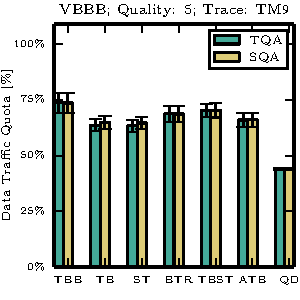
\includegraphics{./gfx/700_VAS/plotSavings_TTTM9_TQ5_PG0_SL2001_BL20000_vid104}}
 \subfloat[][]{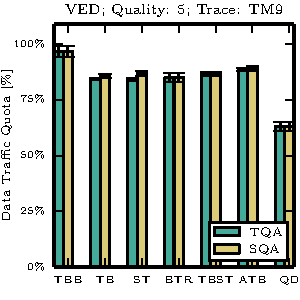
\includegraphics{./gfx/700_VAS/plotSavings_TTTM9_TQ5_PG0_SL2001_BL20000_vid108}}
 \subfloat[][]{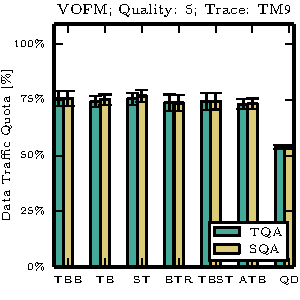
\includegraphics{./gfx/700_VAS/plotSavings_TTTM9_TQ5_PG0_SL2001_BL20000_vid111}}\\
 \subfloat[][]{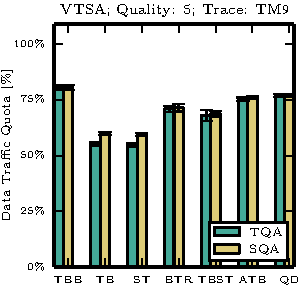
\includegraphics{./gfx/700_VAS/plotSavings_TTTM9_TQ5_PG0_SL2001_BL20000_vid114}}
 \subfloat[][]{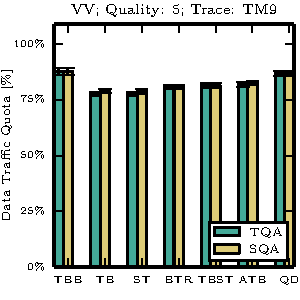
\includegraphics{./gfx/700_VAS/plotSavings_TTTM9_TQ5_PG0_SL2001_BL20000_vid118}}
 \subfloat[][]{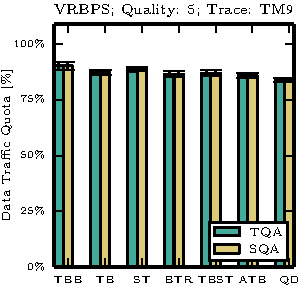
\includegraphics{./gfx/700_VAS/plotSavings_TTTM9_TQ5_PG0_SL2001_BL20000_vid119}}\\
 \subfloat[][]{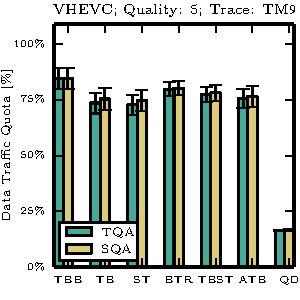
\includegraphics{./gfx/700_VAS/plotSavings_TTTM9_TQ5_PG0_SL2001_BL20000_vid122}}
 \subfloat[][]{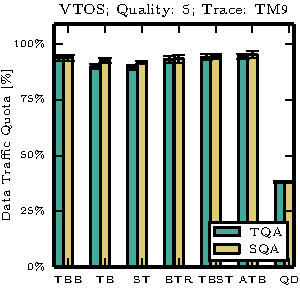
\includegraphics{./gfx/700_VAS/plotSavings_TTTM9_TQ5_PG0_SL2001_BL20000_vid128}}
 \caption[Data traffic quota of VAS for a challenged network trace.]{Data traffic quota of using VAS's TQA and SQA in relation to the pure adaptation scheme for a trace in a challenged network: TM9. The aim is to stream the highest available quality (MOS: 5). The different plots represent the videos VBBB, VED, VOFM, VTSA, VV, VRBPS, VHEVC, and VTOS.}
 \label{fig:730_trafficReductionTM9}
\end{figure}

Figure~\ref{fig:730_trafficReductionTM9} depicts the results of applying \ac{VAS} on the network trace TM9, which contains an average throughput of only 777 \unit{$\frac{KBit}{s}$}.
This is not a sufficient throughput for any of the video sequences to stream the highest bit rate representations at all times.

Note that Figure~\ref{fig:730_trafficReductionTM9} shows the data traffic reductions of \ac{TQA} and \ac{SQA}. 
The differences are minimal as \ac{SQA} is only invoked if an adaptation to a lower quality level is required. 
In comparison to the overall streaming session length, \ac{SQA} is only active for a rather short time.
Thus, only small differences of \ac{TQA} and \ac{SQA} are observed.
A detailed discussion of the \ac{SQA} scheme is given in Section~\ref{sec:730_objectiveQualityVAS}.

\ac{VAS} \ac{TQA} scheme achieves data traffic reductions, even under these challenged conditions, of at least 3.32\% for adaptation scheme \ac{TBB} and the sequence VED, and up to 84.4\% for the video sequence VHEVC and the adaptation scheme \ac{QD}.
For most of the videos (VBBB, VED, VOFM, VRBPS, VHEVC, and VTOS), \ac{QD} benefits most from the application of \ac{VAS}.
This can be explained, as in comparison to the other schemes \ac{QD} risks stalling in a video for the sake of streaming a high quality representation. 
Thus, in challenged network conditions \ac{QD} requests higher bit rate representations.
Thus, the potential for bit rate savings is higher when using \ac{VAS} in comparison to other adaptation schemes.
The other adaptation schemes benefit differently from the \ac{VAS}.

Table~\ref{tab:730_trafficReduction} gives an overview on achievable data traffic savings for the TM3 trace, which has an average throughput of 2.7 \unit{$\frac{MBit}{s}$} and is highly fluctuating over time due to a bus ride with many throughput reductions losses (see Figure~\ref{fig:730_plotTOMMTraces} (b)).
Also, the table shows the average data traffic quota achieved for all network traces.
Again, \ac{QD} benefits most from applying \ac{VAS} in the trace TM3 with data traffic quotas between 16.2\% and 80.4\%.
For TM3 \ac{ATB} shows the lowest data saving potential with a data traffic quota of 94\% for the VRBPS sequence, and thus a saving potential of only 6\%.
Table~\ref{tab:730_trafficReduction} also depicts the average data traffic quotas for different videos (last row) and all adaptation schemes (last column) for all evaluation runs.
The highest saving potential exists for the VHEVC (44\%) and the lowest for VRBPS (19.6\%).
For all traces, \ac{QD} has a data traffic quota of 62.3\% on average, and has the highest potential to save data traffic (37.7\%), whereas \ac{TBB} achieves data saving of 19.2\%.
\begin{table}[htb]
\centering
\caption[Data traffic quota of VAS for different adaptation schemes.]{Data traffic quota of VAS-supported and \ac{VAS}-unsupported adaptation schemes for trace TM3 and aggregated over all traces for all video sequences. The variances or confidence intervals are not shown as the variance is below $10^{-3}$ for TM3 in all cases.} 
\begin{tabular}{l|cccccccc|c}
 \toprule[2.0pt]
 & VBBB & VED & VOFM & VTSA & VV & VRBPS & VTOS & VHEVC & All Videos \\
 \hline
 \multicolumn{9}{l}{TM3} & All Traces\\
 \hline
 TBB&64.6\%&62.8\%&73.4\%&75.3\%&45\%&88.4\%&88.8\%&82.3\%&81.8\%\\
 TB&57.6\%&55.7\%&70.5\%&54.9\%&40.4\%&85.5\%&89.4\%&69.7\%&68.5\%\\
 ST&57.8\%&55.5\%&71.4\%&54.3\%&40.4\%&87.2\%&89.6\%&68.8\%&69\%\\
 BTR&63.4\%&60.6\%&73.1\%&69.7\%&43.4\%&85.8\%&90.3\%&77.6\%&74.3\%\\
 TBSTA&60.7\%&58.6\%&74\%&65.1\%&43.1\%&83.4\%&89\%&75.8\%&73.6\%\\
 ATB&58.7\%&57.9\%&70\%&69.9\%&42\%&83.9&94\%&71.5\%&76.6\%\\
 QD&44.6\%&42.8\%&53.3\%&71.8\%&45.8\%&80.4\%&36.8\%&16.6\%&62.3\%\\
 \hline
 \multicolumn{9}{l}{All Traces}&\\
 \hline
 Avg.&71.7\%&66.3\%&78.5\%&70.5\%&57.3\%&90.5\%&78.7\%&56\%&\textbf{72.3\%}\\
 \bottomrule[2.0pt]
 \end{tabular}
 \label{tab:730_trafficReduction}
\end{table}
On average, \ac{VAS} is able to achieve data traffic savings of 27.7\% independent of the video sequence, adaptation schemes or network trace.
One should note that the traces used in this evaluation represent challenging conditions for mobile video streaming.
Under these difficult conditions, \ac{VAS} achieves considerable data savings across video sequences and adaptation schemes.
These savings are thus higher when inspecting, e.g., the recently available \ac{2160p} videos or network traces from mobile networks with high throughput rates.
\paragraph{How does VAS achieve the savings?}
To better understand achieved data traffic savings, session playback of streaming video with and without \ac{VAS} support is shown in Figure~\ref{fig:730_tracesAndBuffer} for trace TO1. 
\begin{figure}[!h]
 \centering
 \subfloat[][]{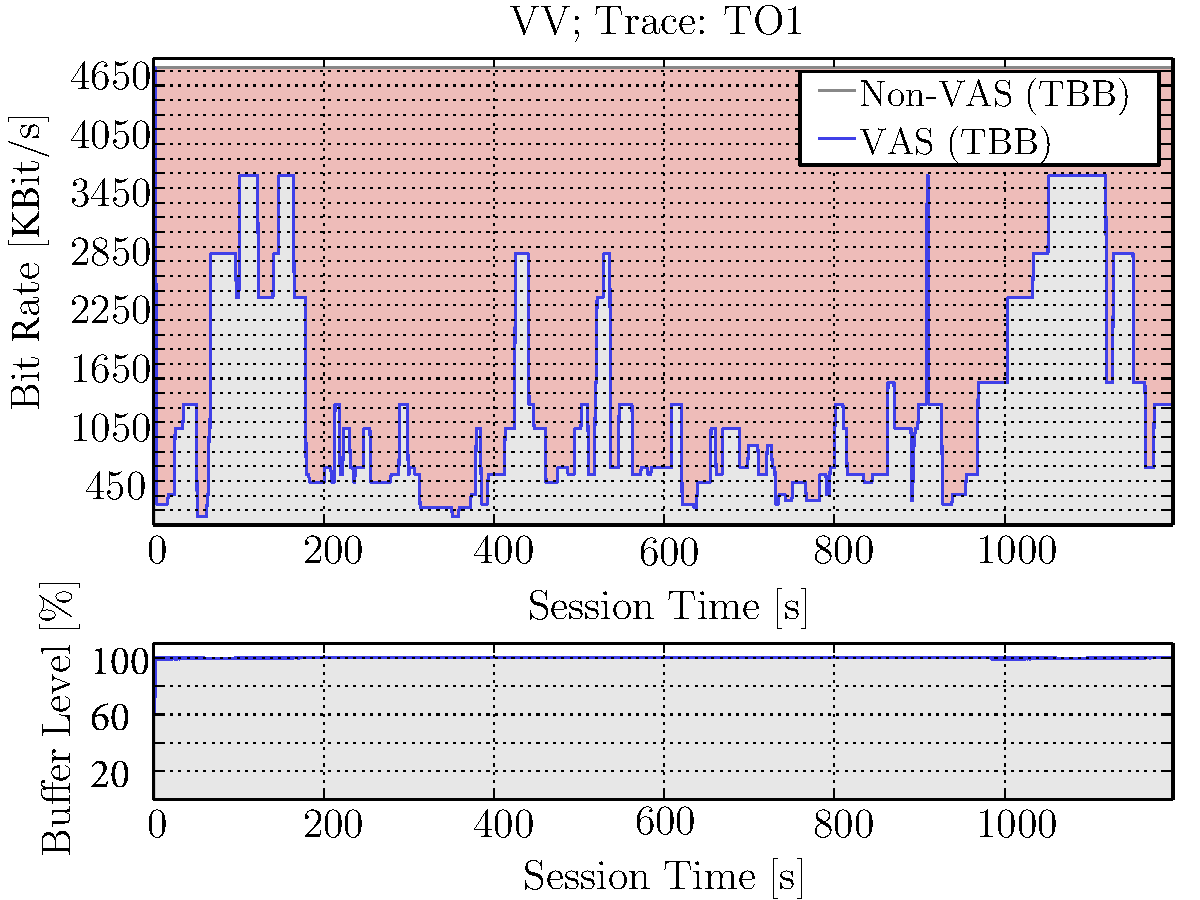
\includegraphics[width=0.49\columnwidth]{./gfx/700_VAS/ploTraceBitrateBuffer_TTTO1_TQ5_PG0_SL2001_BL20000_bt0_SID118}}
 \subfloat[][]{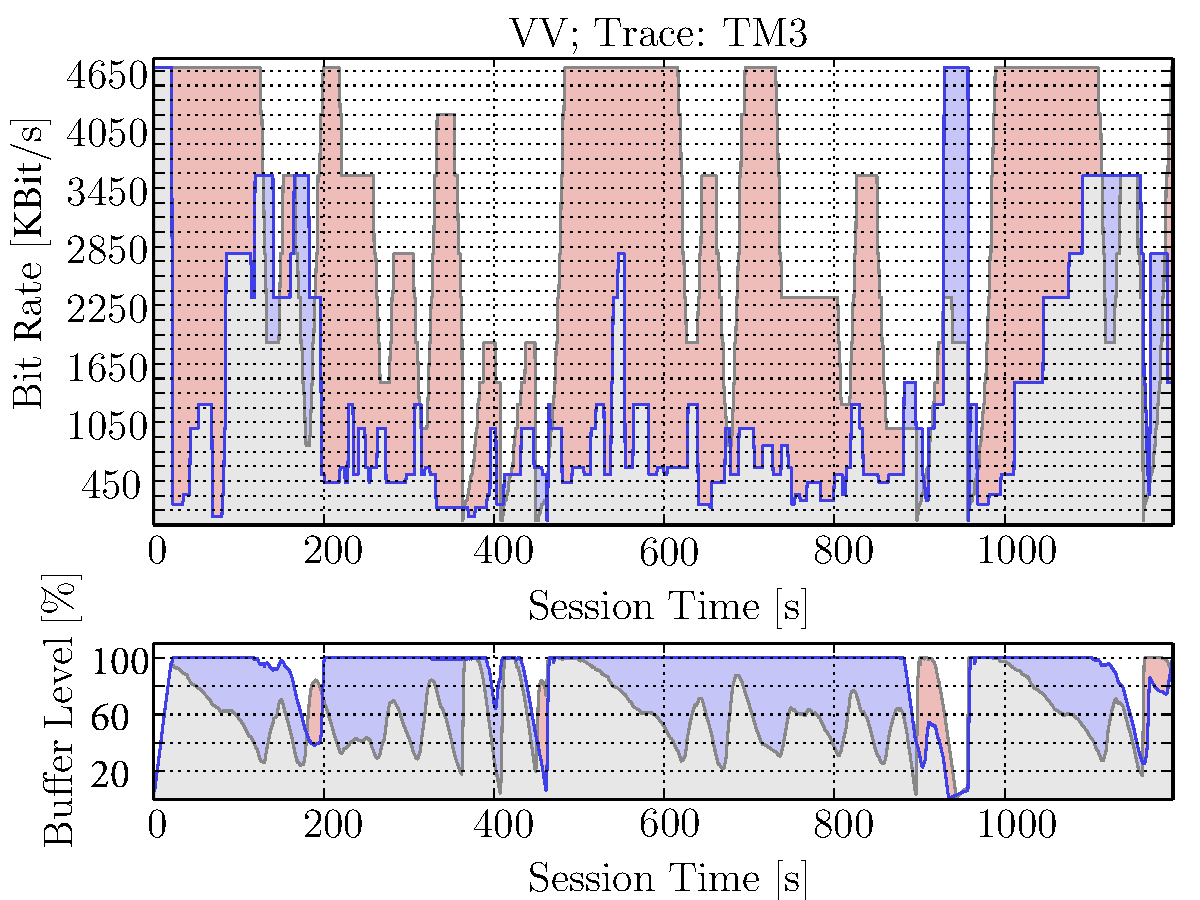
\includegraphics[width=0.49\columnwidth]{./gfx/700_VAS/ploTraceBitrateBuffer_TTTM3_TQ5_PG0_SL2001_BL20000_bt0-SID118}}%
 \caption[VAS session traces for trace: TO1 and TM3]{Comparison of the session traces of the video VBBB for the network traces: TO1 and TM3. In each plot the blue line depicts the bit rate streamed using VAS in comparison to the standard adaptation scheme. A red area indicates throughput savings of the VAS scheme. Plots at the bottom shows the buffer fill rate, where a blue area shows a higher buffer filling rate achieved by VAS.}
 \label{fig:730_tracesAndBuffer}
\end{figure}
For the overcapacity scenario, the \ac{VAS}-unsupported adaptation schemes switch quickly to the highest bit rate available (gray line), whereas \ac{VAS} induces additional adaptations to stream the highest available quality at the lowest possible bit rate.
The red area indicates the achieved data gains over time.
For the trace TM3, \ac{VAS} adapts accordingly and achieves considerable data savings, too.
Another advantage of \ac{VAS} is shown in the buffer statistics of the figure. 
Whereas the classical adaptation scheme runs out of buffer frequently, \ac{VAS} achieves a higher average fill rate of the playback buffer for challenging network conditions (see Figure~\ref{fig:730_tracesAndBuffer} b). 

This principle is illustrated in Figure~\ref{fig:730_timeOnReps} (a).
The figure illustrates a comparison of the session times streamed on different \ac{MPEG} \ac{DASH} representations for the different adaptation schemes with or without \ac{VAS}.
A higher representation index represents a higher bit rate.
It is obvious that in the overcapacity situation, the proportion of lower representations during streaming sessions increases for all videos.
Even for the trace TM3, the time is reduced on higher index representations. 
At the same time, it already indicates (as in the case of TM3) that \ac{VAS} uses saved data traffic to stream higher representations, when the standard adaptation scheme has to stream the lowest representation.
\begin{figure}[!ht]
 \centering
 \subfloat[][]{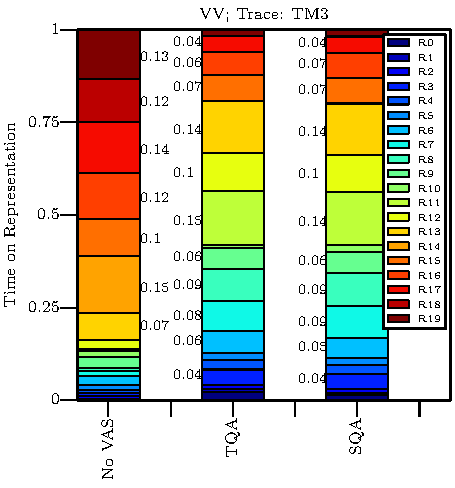
\includegraphics{./gfx/700_VAS/plotRepTimeSingleVideoWithText_TTTM3_TQ5_PG0_bt5_SL2001_BL4000_sID118}}
\subfloat[][]{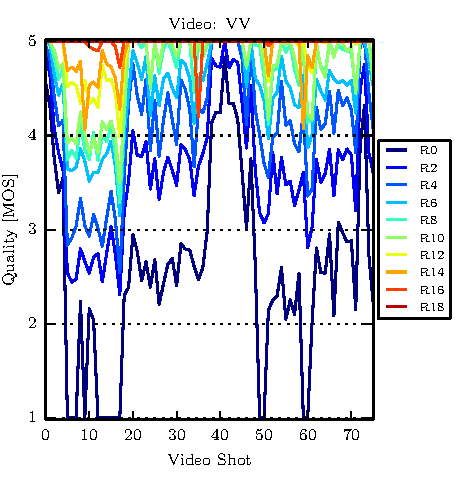
\includegraphics{./gfx/700_VAS/ploVideoQuality_sID118_step_2}}
 \caption[Time on MPEG DASH representation when using VAS]{Time on MPEG DASH representations when using VAS's TQA and SQA scheme for TM3 and video VV: (a) shows a reduced time on higher bit rate representations for all videos in an overcapacity situation (TO1), while (b) shows the achieved quality of different MPEG DASH representations over video shots.}
  \label{fig:730_timeOnReps}
\end{figure}
\paragraph{Influence of SQA on Data Savings}
So far, the results discuss the \ac{TQA} scheme that neglects the influence of \ac{SQA}.
It achieves a perceived quality gain by delaying quality-decreasing adaptations and thus staying longer at higher bit rate representations than \ac{TQA}.
In the case of TO1, \ac{SQA} generates no additional traffic at all.
% SQA: 73 TQA: 72.3
For the remaining traces, e.g., as depicted for TM9 in Figure~\ref{fig:730_trafficReductionTM9}, an average data traffic quota increase of 0.7\% can be observed.

Section~\ref{sec:730_objectiveQualityVAS} and Section~\ref{sec:730_eval_quality} report on the advantages of \ac{SQA} for the perceived quality of a streaming session.
\paragraph{Segment-based Adaptations and Partial HTTP GET Requests}
An additional data traffic reduction can be achieved if the \ac{DASH} client supports partial HTTP GET requests, thus requesting individual byte ranges from a video segment.
This allows adaptation not only at segment boundaries, but also within a \ac{DASH} segment, offering rich potential to adapt for either improved perceived quality or a data traffic reduction. 
Adaptations occur at \ac{GoP} boundaries, but within a \ac{DASH} segment.
A shot boundary could lie within such a segment, resulting in different quality requirements for different parts of the \ac{DASH} segments. 
A partial \ac{HTTP} GET request can extract a byte range from a \ac{DASH} segment that represents an independently decodable frame range, which is determined at encoding time by the \ac{GoP}. 

\begin{table}[htb]
 \centering
 \caption[Partial HTTP GET requests in comparison to the request of segments]{Data traffic quota of VAS-supported and unsupported adaptation schemes for trace TM3, aggregated over all traces for all video sequences. The table depicts the results for both the segment-based HTTP GET requests and partial HTTP GET requests separated by "/".}
\begin{tabular}{l|ccccc|c}
  \toprule[2.0pt]
  \multicolumn{6}{c}{Data Traffic Quota: HTTP GET / partial HTTP GET}& \\
  & VBBB & VED & VOFM & VV & VHEVC & All Videos \\
  \hline
  \multicolumn{6}{l}{Trace:TM3 and TQ: 5} & All Traces\\
  \hline
  TBB&64.6\%/58.8\%&62.8\%/57.4\%&73.4\%/70.1\%&45\%/41.9\%&82.3\%/69.9\%&81.8\%/76.3\%\\
  TB&57.6\%/57.8\%&55.7\%/55.1\%&70.5\%/70.8\%&40.4\%/40.6\%&69.7\%/68.1\%&70.6\%/66.7\%\\
  ST&57.8\%/57.9\%&55.5\%/55.2\%&71.4\%/71.1\%&40.3\%/40.7\%&68.8\%/68.1\%&71.2\%/67.4\%\\
  BTR&63.4\%/58.5\%&60.6\%/56.7\%&73.1\%/70.4\%&43.4\%/41.9\%&77.6\%/65.7\%&74.6\%/73.5\%\\
  TBSTA&60.7\%/58.6\%&58.6\%/56.7\%&74\%/69.6\%&43.1\%/41.8\%&75.8\%/65.1\%&74\%/73.7\%\\
  ATB&58.7\%/58.8\%&57.9\%/56.8\%&70\%/69.2\%&42\%/41.7\%&71.5\%/69.1\%&76.4\%/73.5\%\\
  QD&44.6\%/44.3\%&42.8\%/42.4\%&53.3\%/53.2\%&45.8\%/45.8\%&16.6\%/15.7\%&62.3\%/62.1\%\\
  \hline
  \multicolumn{6}{l}{All Traces and Quality:5}&\\
  \hline
  Avg.&71.7\%/69.1\%&66.3\%/64.1\%&78.5\%/75.3\%&57.3\%/55.7\%&56\%/53.9\%&\textbf{73\%/70.5\%}\\
  \bottomrule[2.0pt]
 \end{tabular}%}
 \label{tab:730_trafficReductionPartialGet}
\end{table}
Table~\ref{tab:730_trafficReductionPartialGet} compares for streaming the videos VBBB, VED, VOFM, VTSA, and VHEVC using \ac{VAS} \ac{TQA} via HTTP 1.1/GET requests (adaptation at segment boundaries only) and partial HTTP 1.1/GET requests (adaptation within segments).
When partial GET requests are used, results indicate a potential of 2.5\% in additional data traffic savings.
In none of the traces or video sequences did partial GET requests decrease the data saving potential.
The impact on the perceived quality is discussed in Section~\ref{sec:730_objectiveQualityVAS}. 
Partial HTTP GET requests can achieve lower data savings, when no potential for additional adaptations exist.
The overhead for using \ac{VAS} with partial HTTP GET is higher, as more requests are sent to the video server and the \ac{VAS} server is consulted more often.
Table~\ref{tab:730_trafficReductionPartialGet} shows two examples.
For video VV and the two adaptation schemes TB and ST the best result is achieved when streaming without partial HTTP GET requests.
%===================================================================================================================================================================
\subsubsection{Achieved Quality during Streaming Sessions}
\label{sec:730_objectiveQualityVAS}
\ac{VAS} aims at stabilizing the perceived quality during streaming while achieving significant data traffic reductions.
For assessing the achieved quality the objective quality assessment metric \ac{RT-VQM} is used~\cite{Wichtlhuber2016}. 
Note, that current video quality assessment metrics do not assess the impact of adaptations.
Assessing the impact of adaptations is evaluated in Section~\ref{sec:730_eval_quality}.

This section describes the effect of \ac{VAS} on the objectively estimated quality by comparing classical adaptation schemes with \ac{VAS} \ac{TQA} and \ac{SQA} schemes, which describes both the influence of video shot-accurate adaptation using partial HTTP GET requests and the influence of \ac{SQA} on stalling.
\paragraph{Different Adaptation Schemes}
The results for determining the average quality per adaptation scheme are illustrated in Table~\ref{tab:730_qualityPreffedAdaptLogicByAL}. This shows an averaged, estimated quality value per adaptation scheme over all network traces and video sequences.
Quality is measured in terms of \ac{MOS}.
The table describes the performance of each adaptation scheme with and without \ac{VAS} support, but neglects additional quality impairments such as adaptation effects (see Section~\ref{sec:730_eval_quality}) and stalling (see Section~\ref{sec:730_eval_stralling}).

It can be observed that significant differences in the qualities of the unsupported adaptation schemes exist. 
Adaptation schemes such as \ac{TBB}, which represent buffer-based decision making, perform worst but in close range to the hybrid scheme \ac{BTR} which represents an extension of \ac{TBB} (difference in \ac{MOS}: 0.02).
Whereas \ac{TBB} solely relies on buffer thresholds for deciding when and how to adapt, \ac{BTR} answers the question of  which representation to switch to using instant throughput estimates.
Solely buffer-based adaptation schemes show the worst performance.
A good performance in terms of improving the average quality of a streaming session is achieved by the adaptation schemes \ac{TB} (\ac{MOS}: 4.17), \ac{ST} (\ac{MOS}: 4.14), and \ac{ATB} (\ac{MOS}: 4.18).
With \ac{TB} and \ac{ST}, two adaptation schemes solely relying on the throughput measurements are proposed, which outperform buffer-based adaptation schemes.
Superior performance is achieved by hybrid models, which integrate both buffer-based and throughput-related adaptation decisions - as \ac{ATB} already shows.
Superior quality is achieved by \ac{TBST} (\ac{MOS}: 4.29) and \ac{QD} (\ac{MOS}: 4.69).
Thus, \ac{QD} and \ac{TBST} especially indicate that considering both metrics, buffer fill state and throughput, can be beneficial.
Additionally, \ac{QD} adds a quality-aware adaptation scheme, which achieves an \ac{MOS} increase of up to 0.4 in comparison to \ac{ATB}. 
In Section~\ref{sec:730_eval_stralling} it is shown that \ac{QD} in particular has significant problems to ensure a stall-free playback.
\begin{table}[htb]
 \centering
 \caption[Perceived quality using the VAS adaptation scheme]{Perceived quality using VAS-supported and unsupported adaptation schemes for the TM3 trace and aggregated over all traces for all video sequences. The variances or confidence intervals are not shown as the variance of the results is below 0.02.} 
 \begin{tabular}{l|cccc|cccc}
  \toprule[2.0pt]
  & \multicolumn{4}{c}{HTTP GET}
    & \multicolumn{4}{c}{Partial HTTP GET} \\
  & \multicolumn{3}{c}{Quality [MOS]}
  & Traffic& \multicolumn{3}{c}{Quality [MOS]} & Traffic \\
  
 & Standard & TQA & SQA & Quota & Standard & TQA & SQA  & Quota\\
  \hline
  TBB & 4.08 &4.36 & 4.35 & 81.8\% & 4.03 & 4.41 & 4.42 & 76.3\% \\
  TB & 4.17 & 4.3 & 4.33 & 70.6\% & 4.15 & 4.3 & 4.41 & 66.7\% \\
  ST & 4.14 & 4.32&  4.36 & 71.2\% & 4.26 & 4.34 & 4.41 & 67.4\% \\
  BTR & 4.1 & 4.29 & 4.33 & 74.6\% & 4.18 & 4.37 & 4.37 & 73.5\% \\
  TBST & 4.29 & 4.31& 4.32 &  74\% & 4.31& 4.39 &4.39 & 73.7\% \\
  ATB & 4.18 & 4.48& 4.5 & 76.4\% & 4.27 & 4.54 & 4.63 & 73.5\% \\
  QD & 4.69 & 4.98& 4.99 &  62.3\% & 4.74 & 4.99 & 4.99 & 62.1\% \\
  \hline
   & 4.23 & 4.43& 4.45 & 73\% & 4.28 & 4.47 & 4.52 & 70.5\%\\
  \hline
  \bottomrule[2.0pt]
 \end{tabular}
 \label{tab:730_qualityPreffedAdaptLogicByAL}
\end{table}

\ac{VAS} support improves the average \ac{MOS} of all adaptation schemes, independent of whether the \ac{TQA} or \ac{SQA} scheme is used.
Especially for challenged network traces, the saved data traffic in times with high throughput can be efficiently used to keep a high buffer fill ratio.
For the adaptation schemes \ac{TBB}, \ac{ATB}, and \ac{QD}, an \ac{MOS} increase of approximately 0.3 is achieved, whereas \ac{TB}, \ac{ST} and \ac{BTR} only benefit from an increase of 0.13 to 0.19.
Both schemes benefit most, as they allow for a rapid increase in the representation index in situations when the measured throughput rises.
The majority of network traces used for the evaluation show throughput increases and decreases due to mobility.
In addition, both schemes slowly decrease representation indexes, thus allowing \ac{VAS} to stream high quality representations over a longer period of time.
By design, \ac{VAS} never recommends a representation, which is higher than the one proposed by the pure adaptation scheme.
The \ac{TBST} scheme achieves the smallest improvement.  
\ac{TBST} by design solely allows for small increases and decreases by one representation index.
Especially for situations with a rapid increase in throughput, \ac{TBST} only slowly improves quality. 
The buffer-based or purely throughput-reliant schemes achieve higher gains.

The introduction of partial HTTP GET requests offers the opportunity to not only adapt at \ac{MPEG} \ac{DASH} segment boundaries.
On the one hand, this allows data traffic reduction by more accurately streaming the desired bit rate by switching within \ac{MPEG} \ac{DASH} segments - bound to an independently decodable \ac{GoP}. 
On the other hand, this allows for improving quality when network conditions rapidly change. 
The adaptation control loop - measuring the buffer fill state, the throughput or both - is more frequently triggered and thus allows for adaptation decisions with a higher precision.
Consequently, the results indicate an increase of 0.19 in comparison to the standard adaptation schemes at a significantly lower data traffic quota - i.e., higher data saving potential.
In comparison to standard adaptation schemes without the support of partial \ac{HTTP} GET requests, an improvement of around 0.29 is observed.
Both results indicate a human-perceivable difference in the resulting video stream.
\paragraph{Comparing TQA and SQA}
For most schemes (see Table~\ref{tab:730_qualityPreffedAdaptLogicByAL}), a rather small improvement can be observed using \ac{SQA} in contrast to \ac{TQA}; this is possible as no direct quality-decreasing switches are introduced but more time is spent on higher representations, which brings the risk of playback buffer depletion.
The average effect for all adaptation schemes lies at approximately 0.02 in comparison to \ac{TQA}.
With the introduction of partial \ac{HTTP} requests, \ac{SQA} achieves a more granular adaptation option when decreasing representation indexes.
As a consequence, \ac{MOS} improvements rise from 0.02 to 0.05 on average, where  especially \ac{TB}, \ac{ST}, and \ac{ATB} benefit most with an average increase of 0.09 in comparison to 0.03 for classical \ac{HTTP} GET.

Based on the aforementioned results: In comparison to \ac{TQA}, a superior \ac{SQA} performance can be observed for most adaptation schemes using HTTP GET requests and for all using partial HTTP GET requests.
\paragraph{Influence of Stalling}
\label{sec:730_eval_stralling}
Previous discussions report on the advantage of \ac{VAS} as measured in terms of perceived qualities averaged for the streaming session, neglecting stalling effects.
Different adaptation schemes may more or less efficiently avoid playback buffer underruns. 
Thus, Table~\ref{tab:730_qualityPreffedAdaptLogicIncludingStalling} depicts in the "Standard" column the average quality achieved when using an adaptation scheme and the impact of occurring stalls during streaming sessions as well as the resulting quality scores.

For estimating the impact of stalls, the model of Mok et al.~\cite{Mok2011} integrates the mean stalling time ($L_T$) and the frequency ($L_{FR}$) of stalls in a time window of about 90 seconds, and measures the impact in large subjective studies for \ac{HAS}.
The model was explained in Section~\ref{sec:250_stalling_video}.

Table~\ref{tab:730_qualityPreffedAdaptLogicIncludingStalling} depicts the quality scores estimated by the objective quality assessment metric, the effect of stalling on the perceived quality and  and the resulting quality scores. 
The table shows only the results of partial \ac{HTTP} GET requests as it is superior for \ac{VAS}-assisted adaptation.
For standard adaptation schemes, an initial surprise is a significantly reduced quality achieved by \ac{QD}. 
Even though it is designed to support quality-aware adaptation, its design does not reliably avoid stalling.
It achieves streaming high quality representations at the cost of risking stalls. 
In contrast, a superior performance can be observed for \ac{ATB}, \ac{ST}, and \ac{TBST} (\ac{MOS} of 4.07, 4.07 and 4.12).
In general, the stalling impact is rather low when averaged over all sessions.
On average, the \ac{MOS} decreases by 0.38 when averaged across all adaptation schemes. 

\begin{table}[htb]
 \centering
 \caption[Influence of stalling on the perceived quality using VAS]{Influence of stalling proposed by Mok et al. on the quality scores for using VAS's TQA and SQA schemes in comparison to standard adaptation schemes. Results solely depict streaming sessions using partial HTTP GET results.}
 \begin{tabular}{l|ccc|ccc|ccc}
  \toprule[2.0pt]
   & \multicolumn{3}{c}{Quality [MOS]}
   & \multicolumn{3}{c}{\specialcell{Stalling Effect [MOS] \\by Mok~\protect\cite{Mok2011}}} &  \multicolumn{3}{c}{Quality Score [MOS]} \\
   & Standard&TQA&SQA&Standard&TQA&SQA&Standard&TQA&SQA \\
  \hline
  TBB & 4.03 & 4.41 &4.42 & 0.17 & 0.11 & 0.1 & 3.86& 4.3  & 4.32 \\
  TB & 4.15 & 4.3 & 4.41 & 0.19 & 0.08 & 0.08 & 3.96 & 4.22 & 4.33 \\
  ST & 4.26 & 4.34 & 4.41 & 0.19 & 0.08 & 0.09 & 4.07& 4.26  & 4.32 \\
  BTR & 4.18 & 4.37 & 4.37 & 0.18 & 0.09 & 0.09 & 4.00 & 4.28 & 4.28 \\
  TBST & 4.31& 4.39 & 4.39 & 0.19 & 0.06 & 0.06 & 4.12 & 4.33 & 4.33\\
  ATB  & 4.27 & 4.54 & 4.63 & 0.2 & 0.05 & 0.05 & 4.07 & 4.49 & 4.58\\
  QD & 4.74 & 4.99 & 4.99 & 1.51 & 1.4 & 1.42 & 3.23 & 3.59 & 3.57 \\
  \hline
  & 4.28 & 4.47 & 4.52 & 0.38 & 0.26 & 0.27 & 3.9 &4.21 & 4.25 \\
  \hline
  \bottomrule[2.0pt]
 \end{tabular}
 \label{tab:730_qualityPreffedAdaptLogicIncludingStalling}
\end{table}
The resulting impact of stalling is reduced using \ac{VAS} by an \ac{MOS} of 0.12 when applying \ac{TQA} and around 0.11 using \ac{SQA}.
These quality improvements are an additional side effect of \ac{VAS}'s bit rate savings, which can now ensure more stable playback of a video stream.
In situations when the available throughput is scarce, any saved bit can be leveraged to ensure a suitable fill rate of the playback buffer. 
An example is given in the previous section in Figure~\ref{fig:730_tracesAndBuffer} (b).
The figure shows that due to saved data traffic over a long period of time, the buffer level can be kept at 100\%, whereas the standard \ac{MPEG} \ac{DASH} adaptation schemes encounter stalling.
Thus, the number and duration of stalls decrease, resulting in a reduced impact of stalling when \ac{VAS} is used. This improvement can be observed for any adaptation scheme.
The slightly worse performance of \ac{SQA} in comparison to \ac{TQA} is related to the risk of delaying decreasing adaptations, at the risk of additional stalling. 
For five of the seven adaptation schemes, no additional stalls using \ac{SQA} could be observed.
However, the average quality, including stalling events, is approximately 0.04 higher than in \ac{TQA}.
The effect of adaptations on the perceived quality is not considered, it is discussed in Section~\ref{sec:730_eval_quality}.
In particular, the adaptation schemes reacting quickly to a throughput benefit most from applying \ac{VAS}, i.e., hybrid and throughput-based adaptation schemes.

But independent of the adaptation scheme used, \ac{VAS} improves the streaming experience by increasing the average quality of the streamed representations and stabilizing the buffer fill ratios which avoids \ac{stalling}. 
%================================================================================================================================================
\subsection{Subjective Studies on the Impact of Adaptations}
\label{sec:730_eval_quality}
The \ac{VAS} service may introduce additional adaptations between different \ac{MPEG} \ac{DASH} representations.
Table~\ref{tab:730_qualityPreffedAdaptLogicByAL} indicates that the \ac{VAS} \ac{SQA} scheme achieves a slight increase in the objectively measured video quality. 
Note that the impact of an adaptation on the perceived quality is not measured by an objective video quality metric.
In contrast to classical \ac{MPEG} \ac{DASH} adaptation schemes, \ac{VAS} respects the content properties; also \ac{SQA} is capable of leveraging intermediate representations when switching between quality levels.

As available quality metrics do not yet consider adaptation effects, subjective studies are conducted to analyze the real gains when using \ac{SQA}.
\ac{SQA} is investigated in respect of the perceived quality when users watch an adaptive video.
Adaptations at segment boundaries (\ac{HTTP} GET requests) and at shot boundaries (partial \ac{HTTP} GET requests) are compared in terms of their effect on human perception.
The subjective study includes 23 test subjects watching selected video segments on a mobile device mediated by the crowdsourcing platform Crowdee\footnote{http://crowdee.de allows for conducting crowdsourcing studies on mobile devices; Visited on: 09/25/2016}.
The users' age ranged from 17 to 34. 18 of the assessors are male.
The \ac{SQA} smooth adaptation scheme is compared with the standard \ac{TB} adaptation scheme. 
The maximum duration of each video segment used in this evaluation is a 30 $\unit{seconds}$.
It represents adaptations induced by the trace TM2 with a difference from the source to the target representation index of at least five index steps.



The differences in perceived quality are determined using the \ac{JND}~\cite{Watson2001} in combination with a forced choice experiment, as described in Section~\ref{sec:210_subjective_quality}.
Adaptation assistance is evaluated by using three sequences: stable subjective quality, and the increase and decrease of quality.
The video sequence selection is made based on varying \ac{SI}, \ac{TI}, and \ac{Co} characteristics.
Figure~\ref{fig:730_eval_subjective} shows the results of the subjective study in terms of the absolute \ac{JND}.
\begin{figure}
\centering

\subfloat[]{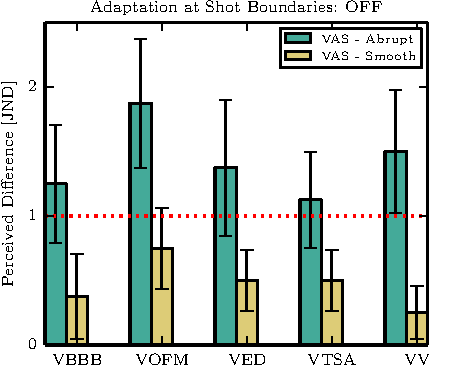
\includegraphics{./gfx/700_VAS/plotMOS_TT0}}
\subfloat[]{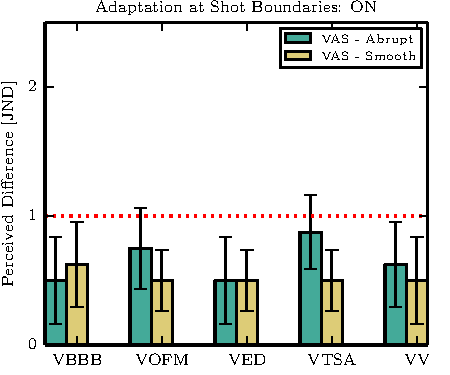
\includegraphics{./gfx/700_VAS/plotMOS_TT1}}
\caption[Perceived quality measured by the JND using VAS]{ 
Perceived quality measured by the \ac{JND} when using the \ac{VAS} \ac{SQA} ensuring a consistent quality placing the adaptations (a) at segment boundaries and (b) at video shot boundaries.}
\label{fig:730_eval_subjective}
\end{figure}
In a second step, the difference is determined for the perceived quality between a video streaming session that keeps a high bit rate representation. 
The analyzed situation is when a stable perceived quality results in a significant decrease of the \ac{MPEG} \ac{DASH} representation index. This gives an impression on how the impact of the adaptation is perceived. 
The experiment is conducted for all five video streams from which eight segments of at most 30 seconds are extracted.
\ac{VAS} performs \ac{MPEG} \ac{DASH} representation adaptations to ensure a stable perceived quality experience while minimizing data traffic. 
During the evaluation, it is ensured that no quality-degrading effects occur other than the adaptation (e.g., stalling or packet loss induced artifacts). Each subject has to evaluate 24 randomly selected combinations containing a reference video with a stable bit rate, and a video sequence using either  \ac{SQA} or \ac{TQA}.

In addition, video  adaptation schemes are placed either at \ac{MPEG} \ac{DASH} segment boundaries (see the results in Figure~\ref{fig:730_eval_subjective} a) or at the shot boundaries detected by \ac{VAS} (see Figure~\ref{fig:730_eval_subjective} b).
The depicted results give an idea on which adaptations are perceivable by humans.
A \ac{JND} of one is depicted as a red barrier when it is assumed that an adaptation is strongly perceivable by human observers on a mobile device.
 
For the case where adaptations are executed only after a complete \ac{MPEG} \ac{DASH} segment was played back (as evaluated in Figure~\ref{fig:730_eval_subjective} a), users notice considerable quality differences. 
It can be concluded that abrupt switches between a source and a target representation are observable on a mobile device.
The \ac{VAS} smooth adaptation scheme decreases the \ac{JND} for the video sequences VBBB, VOFM, VED, and VV significantly.
If the \ac{MPEG} \ac{DASH} client supports partial GET requests, adaptations should be planned to be executed at shot boundaries as this makes the adaptation transparent to the user.
Executing adaptations at shot boundaries allows for adjusting the bit rate of the video stream with abrupt switches, which are nearly imperceivable for VBBB, VED, and VV. 
It can be concluded that \ac{VAS} smooth adaptation ensures that for most evaluated videos, adaptations can be executed in a nearly imperceivable manner. 
